\section{Extension to Higher Dimensions}\label{sec:mud-higher-dimensions}
We present a scenario to further underscore the value of considering geometry when constructing a QoI map for use in solving a SIP to perform parameter identification.
We show that when the dimension of $\pspace$ is higher, the benefit from maximizing the dimension of $\dspace$ is even more considerable than what we observed in the two-dimensional cases.
In the second example, we illustrate how we could use the solution to the SIP for the two-dimensional case from \ref{subsec:pde-example} to better construct the problem we pose in five dimensions.
In particular, we show the effect that this refinement of a 5-D parameter space has on the estimated boundary--condition functions $\widehat{g}$ induced by the MUD solutions to the 5-D SIP.

Suppose that an experimenter less familiar with parameterization of curves and the problems associated with high-dimensions decided to start with a five--dimensional problem (five knots to describe $g$ instead of two), trying to accomplish greater granularity in the ability to estimate $g$, and imposes the same type of uniform initial density in each direction, yielding a parameter space of $\pspace = [-4, 0]^5$.
In Figure~\ref{fig:pde-highd-initial}, we show what such initial functions would look like, and note that many of them appear to exhibit fluctuating behavior for which the mesh ($36\times36$) being used to solve the problem, would not be fine enough to resolve.
This choice of initial density induces a lot of noise into the SIP we are hoping to solve, since ``common sense'' from a modeler's perspective could rule out zig-zag functions from wasting a model-evaluation budget, which we fix at the same $N=1000$ samples as in the previous 2-D problems.
We address one way these observations can be incorporated into posing a better SIP in the next example.
To establish a baseline for what we could expect the best possible representations in this peculiar choice of ``basis'' could be, we again find the closest match to the interpolating and to the noiselesss measurement data and plot them alongside residuals in Figure~\ref{fig:pde-5d-proj}.

\begin{figure}
\centering
  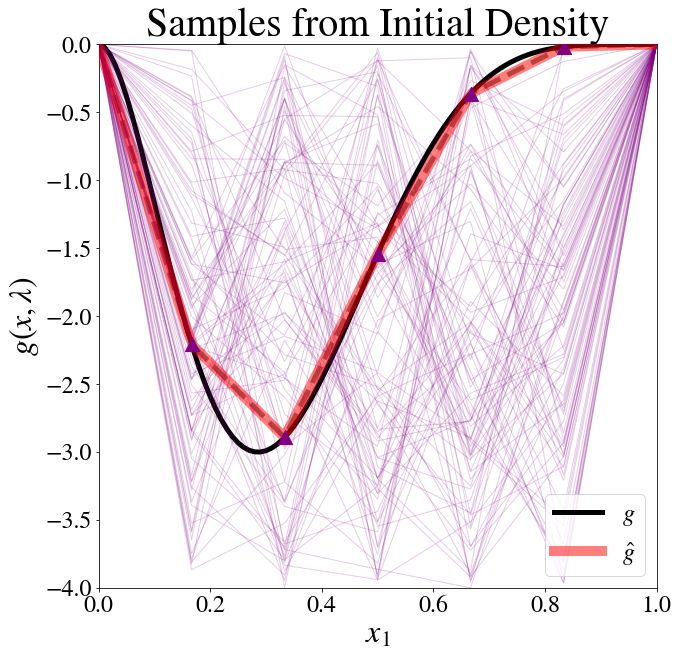
\includegraphics[width=0.475\linewidth]{figures/pde-highd/pde-highd_init_D5.png}
\caption{
One thousand initial parameter samples (our model evaluation ``bugdet'') were used to estimate $g$, constructed by taking independent uniform samples from $[-4, 0]$ for each direction are shown in purple.
}
\label{fig:pde-highd-initial-5d}
\end{figure}


\begin{figure}[htbp]
\centering
  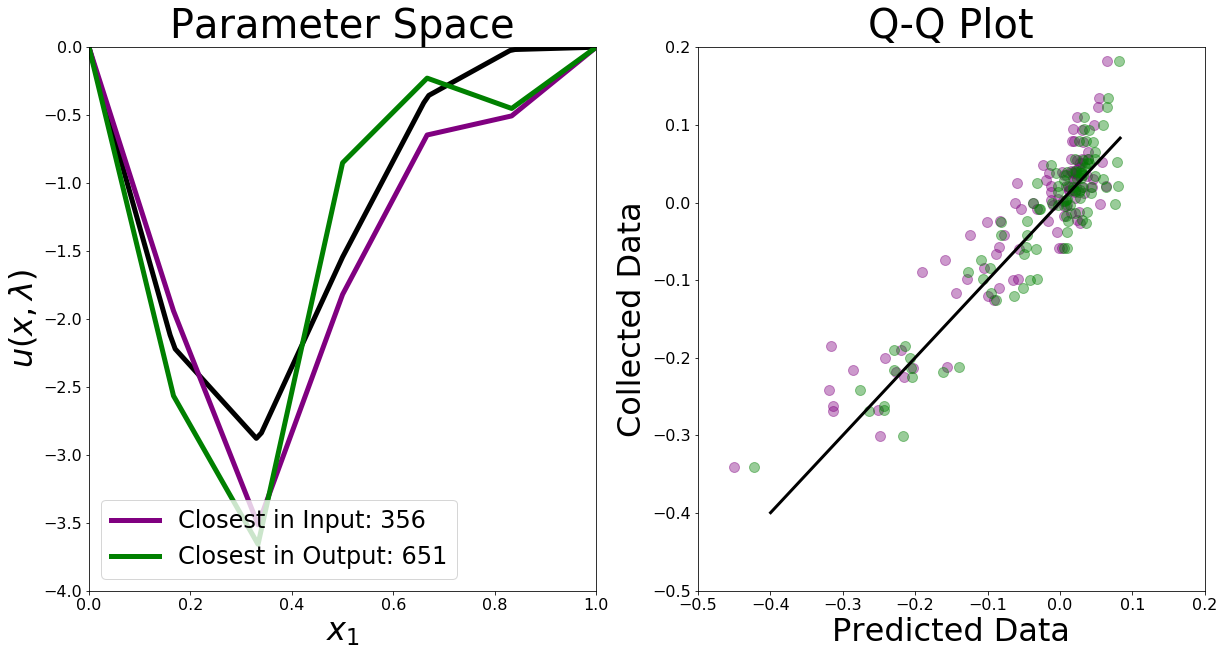
\includegraphics[width=0.675\linewidth]{figures/pde-highd/pde-highd_proj_D5}
\caption{
}
\label{fig:pde-5d-proj}
\end{figure}

Observe that in Figure~\ref{fig:pde-5d-proj}, both the closest fit in parameter and measurement space fail to resolve the true function behavior at $\lambda_5$ (the interpolating piecewise--linear is shown again for reference), and both place a minimum at $\lambda_2$.
The lines here are in some sense, the best that can be solved for with this design, and is helpful for comparing against our MUD solutions.
Of particular interest is that both functions under-estimate $g$ at $\lambda_2$ by a large margin.
Nevertheless, we pursue the solution for demonstration purposes and solve the SIP for both scalar-- and vector--valued QoI maps, the latter constructed with horizontal bands shown in the bottom left of Figure \ref{fig:pde-highd-5d-example}.

\begin{figure}[htbp]
\centering
  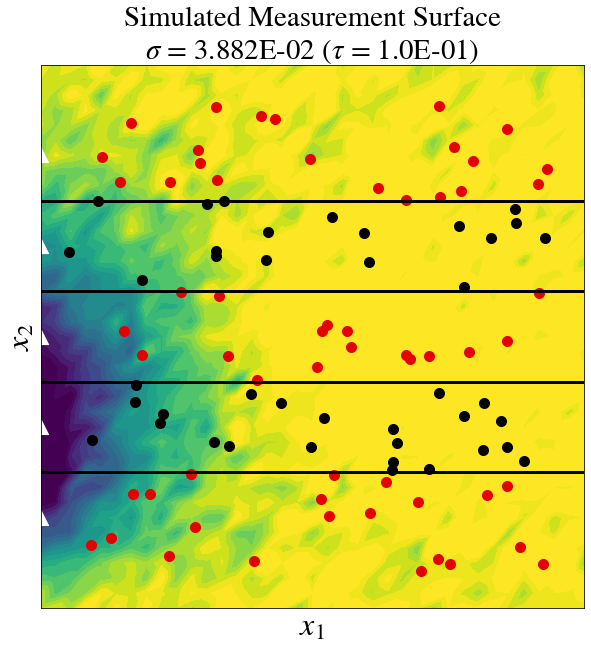
\includegraphics[width=0.35\linewidth]{figures/pde-highd/pde-highd_sensors_D5}
  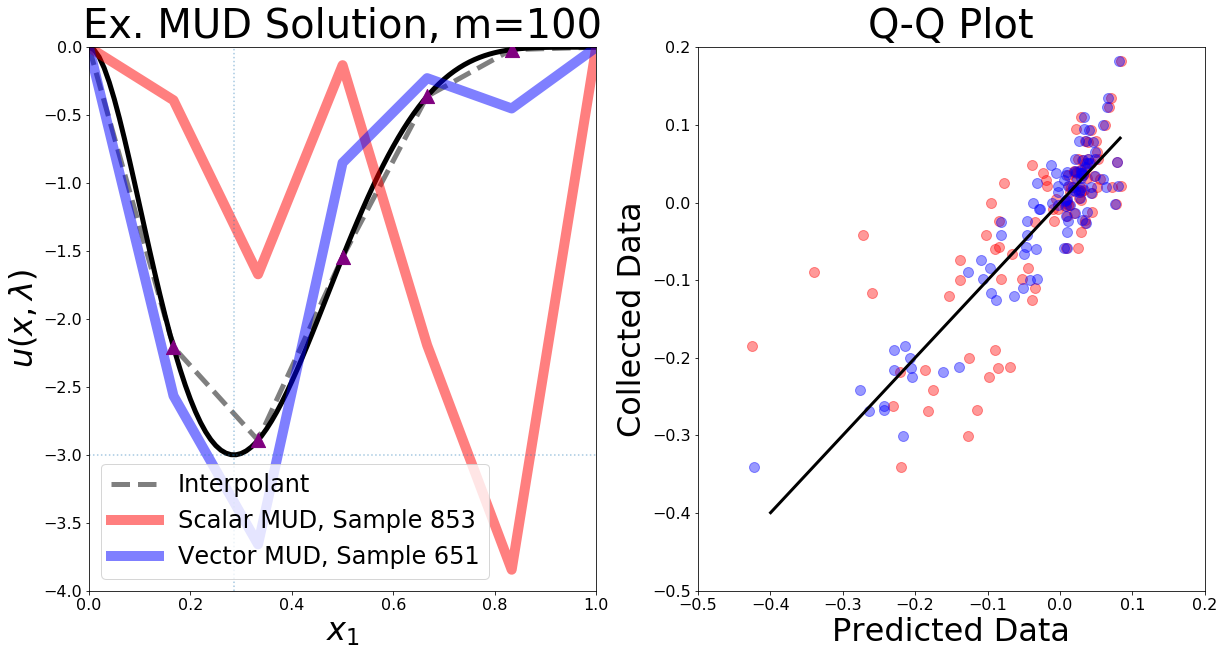
\includegraphics[width=0.6\linewidth]{figures/pde-highd/pde-highd_comp_exmud_D5_m100}
\caption{
(Top): Layout for 5-D vector--valued map and comparison of the two MUD solutions in parameter space.
(Bottom): The response surfaces predicted by the two QoI maps alongside the noisy response surface that generated the simulated collected data.
}
\label{fig:pde-highd-5d-example}
\end{figure}

In Figure~\ref{fig:pde-highd-5d-example}, the scalar-- and vector--valued MUD solutions are shown for the noisy surface plotted in the top-center, with associated predicted response surfaces flanking it.
In the bottom-center plot, we can see that the scalar-valued MUD completely misidentifies the location of $g$'s minimum value, but the vector-valued QoI is able to resolve the behavior much better.
In Figure~\ref{fig:pde-highd-5d-mud} we plot the results from twenty repeated trials (perturbations of noise) when using all hundred measurements, and observe the same difference in going from scalar-- to vector--valued solutions for the 75--dimensional example that we saw in 2 dimensions with \ref{fig:pde-MUD}\footnote{See Appendix~\ref{app:pde-example} for examples of the twenty MUD-solutions using different numbers of measurements.}.

\begin{figure}[htbp]
\centering
  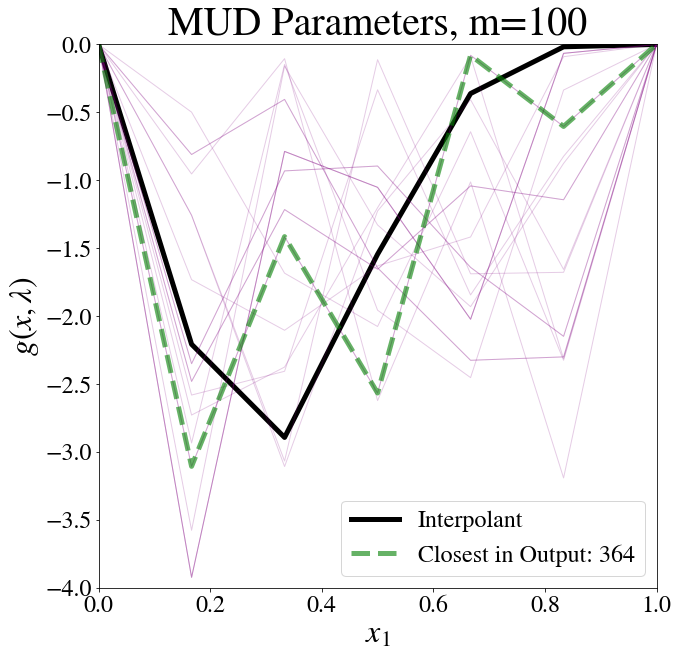
\includegraphics[width=0.95\linewidth]{figures/pde-highd/pde-highd_pair_D5-1_m100}
  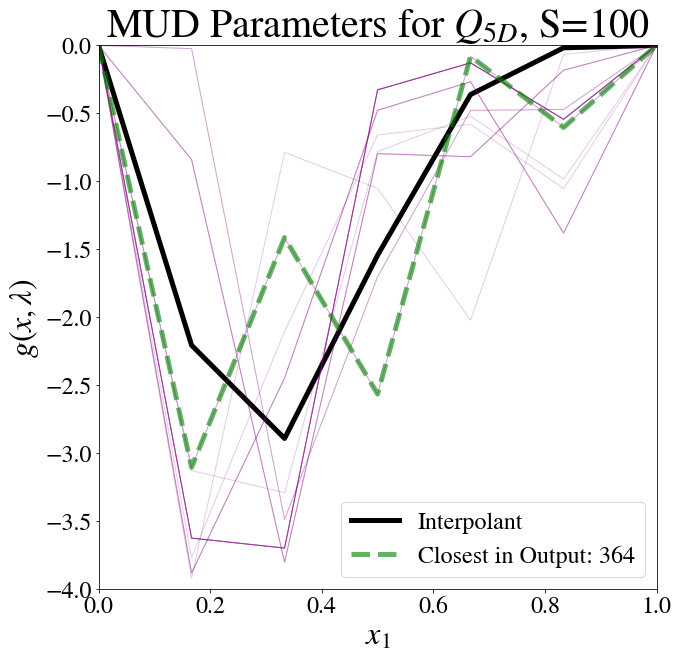
\includegraphics[width=0.95\linewidth]{figures/pde-highd/pde-highd_pair_D5-5_m100}
\caption{
(Top): Scalar-valued solutions.
(Bottom): Vector-valued solutions.
}
\label{fig:pde-highd-5d-mud}
\end{figure}

By increasing the number of QoI, more directions of uncertainty are resolved in the parameter space.
Since any solution in the equivalence class is valid for the SIP, the scalar-valued solutions are significantly more sensitive to noise, and so the solutions often appear to identify functions with a minimum on the wrong half of the spatial domain.
In the left half of Figure~\ref{fig:pde-highd-5d-mud}, the scalar-valued QoI is unable to differentiate between resolving residual discrepancies in different locations in $\Omega$.
By contrast, the vector-valued QoI shown below it is again constructed with respect to the flow of information in the system, and so many more of the twenty trials land closer to the true minimum value of $g$.
The solutions for the vector-valued approach instead explore the available knots (at $x_2=1/6$ and $1/3$), nearest the actual minimum value of $2/7$ instead, a much more valuable area of $\Lambda$ to explore.

Perhaps unsurprisingly given the poorly-designed initial density (equal intervals for each parameter), our MUD solutions still do not really trace out the interpolants or projections from Fig~\ref{fig:pde-5d-proj} that it should to approximate $g$.
At the very least, we would hope to accurately estimate the location and value of $g$'s minima.
Recall from \ref{subsec:pde-example} that we previously solved a two-dimensional version of this problem, which could have been used to inform a much smaller region of two of the five directions to explore.
We now explore what would happen if our initial density was constructed with more care (without needing to use any model evaluations), since we saw from earlier examples that if DCI is initialized at a good initial mean, it has a chance of outperforming least-squares solutions in resolving discrepancy in truth.
